\documentclass{meta}
\usepackage{amsmath,amssymb}
%\usepackage{amsthm}
\usepackage{graphicx}
%\usepackage{graphics}
%\usepackage{algorithm}
%\usepackage{tikz,tkz-tab}
\usepackage[normalem]{ulem}
\usepackage[utf8]{inputenc}
\usepackage{pgfplotstable}
\usepackage{pgfplots}
\usepackage{changepage}
\useunder{\uline}{\ul}{}


\def\N{{\mathcal{N}}}
\def\NN{{\mathbb{N}}}
\def\ZZ{{\mathbb{Z}}}
\def\RR{{\mathbb{R}}}
\def\un{{\rm{1\!\!1}}}
\def\CC{{\mathcal{C}}}
\def\HH{{\mathcal{H}}}
\def\UU{{\mathcal{U}}}
\def\II{{\mathcal{I}}}
\def\JJ{{\mathcal{J}}}
\def\TT{{\mathcal{T}}}
\def\PP{{\mathcal{P}}}
\def\SS{{\mathcal{S}}}
\def\WW{{\mathcal{W}}}
\def\KK{{\mathcal{K}}}
\def\MM{{\mathcal{M}}}

 
\begin{document}
\title{Rapport TER Clustering in a 2D pareto front}

\author{A. Gallot, A. Chesneau}


\institute{Université Paris-Sud, Orsay, France \\ \email{antonin.gallot@u-psud.fr,adrien.chesneau@u-psud.fr}}

\maketitle

\section{Introduction}

Ce rapport a été écrit pour le TER: Clustering, une initialisation à la recherche sur les travaux de Nicolas Dupin, Frank Nielsen et El-Ghazali Talbi, "Dynamic Programming heuristic for $k$-means Clustering among a $2$-dimensional Pareto Frontier".
Où notre groupe doit tout d'abord s'informer sur l'état de l'art général avant d'approfondir ce travail via 4 approches différentes:\\
-Optimisation exacte, algorithmique et programmation.\\
-Programmation parallèle.\\
-Design et comparaison entre approches heuristiques.\\
-Questionnement sur l’impact du choix des mesures de clustering.

\section{Etat de l'art général}

Les problèmes de clustering de données sont en général NP-Dur dans $\mathbb{R}^2$. Mais le fait d'être dans un front de pareto donne une propriété specifique : \\
$C_{i,i'}={\{x_j\}_{j\in [i,i']} = \{ x \in E | \exists j \in [i, i'], x = {x_j} \}$.\\
Autrement dit, les calculs des $C_{i, i'}$ sont polynomiaux, ce qui implique l'existence d'un algorithme de programmation dynamique polynomial. C'est de cet algorithme de programmation dynamique que nous allons partir.

\subsection{Générateur d'instances}

Nous avons commencé par faire un générateur d’instances aléatoires représentant les points sous un front de Pareto en 2 dimensions. Ce générateur comprend 4 fonctions:\\
-dataConvex tire un nombre $N$ de points entre $[a,b]$ qui sont fractionnés avec $f_{a,b,\alpha}:x\in[a,b]-> \frac{1}{x^\alpha}$ avec $\alpha>0,0<a<b$ puis triés dans l'ordre croissant. Cela permet d'avoir une distribution des points bien répartie.\\
-dataConcav tire un nombre $N$ de points entre $[a,b]$ qui sont soustraits avec $f_{a,b,\alpha}:x\in[a,b]-> 1000-x^\alpha$ avec $\alpha>0,0<a<b$ puis triés dans l'ordre croissant.\\
-dataAlea tire un premier point $(0,1000)$ puis tire 2 valeurs $a,b>0$ indépendantes sur des bornes $a\in]0, A], b\in]0, B]$ qui sont utilisées pour le point $(0+a,1000-b)$. On ré-itère $N$ fois avec pour un point
$(a_{n},b_{n})$, on construit avec $a_{n+1}=a_{n}+a,b_{n+1}=b_{n}-b$ en respectant les bornes de $a,b$.\\
-dataAleaBox où on initialise une liste de boîtes $L$ avec initialement un seul élément $[0,1000]×[0,1000], n=0$ nombre de points construits, $F$ une liste de points initialement vide. Tant que $n<N$:
On choisit aléatoirement une boîte dans $L$ : boîte $[a,b]×[c,d]$.
On tire aléatoirement un point $x$, $y$ dans la boîte $[a,b]×[c,d]$ que l’on insère dans $F$.
On remplace la boîte $[a,b]×[c,d]$ dans $L$ par les deux boîtes $[a,x]×[y,d]$ et $[x,b]×[c,y]$.
Enfin, on trie la liste $F$ si ce n’était pas le cas (construction par insertion triée).\\

\subsection{Méthode de partitionnement de données}

Nous avons aussi codé les différentes fonctions de mesure de coût de clustering: 

K-means: $f_{means}(Ci,i')=\sum_{I=i}^{i'} ||x_{I}-\frac{1}{i'-i+1}\sum_{j=i}^{i'} x_{j}||^2$\\ \\ 
K-medoids: $f_{medoids}(Ci,i')=$min$_{I\in[i;i']}\sum_{j=i}^{i'} ||x_{j}-x_{I}||^2$\\ \\ 
K-median: $f_{median}(Ci,i')=$min$_{I\in[i;i']}\sum_{j=i}^{i'} ||x_{j}-x_{I}||$\\ \\ 
discrete K-center: $f_{ctr}^{D}(Ci,i')=$min$_{j\in[i;i']}$max$(||x_{j}-x_{i}||,||x_{j}-x_{i'}||)$\\ \\ 
continuous K-center: $f_{ctr}^{C}(Ci,i')= \frac{1}{2}||x_{i'}-x_{i}||)$\\

\subsection{Programmation dynamique}
Enfin, nous avons codé l'algorithme de programmation dynamique suivant:

\begin{figure}[ht]
 \centering 
\begin{tabular}{ l }
\hline
\textbf{Algorithm 1: $k$-means clustering in a 2d-Pareto Front}\\
\hline
\verb!  !\\

\textbf{Input:} \\
%- \verb!Pblm! a problem amon,g $k$-means, p-center, p-median,\\
- $N$ points  of $\RR^2$, $E =\{x_1,\dots, x_N\}$  %fulfilling hypothesis (\ref{hypoNonDominated})
such that for all $ i\neq j$, $x_i \phantom{0} \mathcal{I} \phantom{0} x_j$ ;\\
- $K\in\NN$ the number of clusters\\

\verb!  !\\

\textsc{Cluster2dPareto}(E,K)\\
\verb!  ! //Initialization phase. \\ %of matrices $c$ and $C$.\\
%\textbf{Initialization:}\\ % \verb!currentSolution = null!, %$\mathcal{N}=$initial neighbourhood.\\
\verb!  ! define matrix $c$ with $c_{i,j}=0$  for all $(i,j)\in [\![1;N]\!]^2$\\
\verb!  ! initialize  matrix $C$ with  $C_{i,k}=0$  for all $i\in [\![0;N]\!], k\in [\![1;K]\!]$\\
\verb!  ! initialize $\PP=$\verb!nil!, a set of sub-intervals of $[\![1;N]\!]$.\\
%\textbf{Initialization:}\\
\verb!  ! sort $E$ following the order of Proposition \ref{reord}\\
\verb!  ! compute $c_{i,j}$ for all $(i,j)\in [\![1;N]\!]^2$ as in section \ref{sec::singleCluster}\\
\verb!  ! //Construction of the matrix $C$ \\
\verb!  ! \textbf{for} $i=1$ to $N$\\

\verb!    ! // case $k=1$ treated separately\\
\verb!    ! set $C_{i,k} = c_{1,i}$\\
\verb!    ! \textbf{for} $k=2$ to $K$ \\
\verb!      ! set $C_{i,k} = \min_{j \in [\![1,i]\!]} C_{j-1,k-1} + c_{j,i}$\\
\verb!    ! \textbf{end for} \\
\verb!  ! \textbf{end for} \\
\textbf{return} $C_{N,K}$ the optimal cost \\

\verb!  ! //Backtrack phase\\
\verb!  ! $i=N$\\
\verb!  ! \textbf{for} $k=K$ to $1$ with increment $k \leftarrow k-1$\\
\verb!    ! find $j\in [\![1,i]\!]$ such that $C_{i,k} = C_{j-1,k-1} + c_{j,i}$\\
\verb!    ! add $[\![j,i]\!]$ in $\PP$\\
\verb!    ! %\textbf{if} $j>1$ \textbf{then}
$i=j-1$\\
\verb!  ! \textbf{end for} \\

\textbf{return} the partition $\PP$ giving the cost $C_{N,K}$\\
\hline
\end{tabular}
\end{figure}

Qui nous donne premièrement la matrice de coût $C_{i,k}$ avec $i$ le nombre de points et $k$ le nombre de cluster. Puis secondement, la backtrack nous donne les coûts qui ont permis de trouver le coût $C_{i,k}$, ce qui permet de retrouver les clusters.

\section{Problématique}

L'objectif de notre TER est de mettre en place des heuristiques afin de trouver les meilleurs compromis entre la qualité des solutions données par ces heuristiques par rapport à la programmation dynamique et le temps de calcul, général ou spécifique à une mesure de clustering particulière.\\
Plus spécifiquement parmi les heuristiques, nous avons choisi de comparer l'algorithme de programmation dynamique avec un autre algorithme de clustering, l'algorithme de Lloyd. L'algorithme de Lloyd ne donne pas la solution optimale mais son temps de calcul, en fonction de ses paramètres de seuil et de nombres d'itérations maximales, est bien plus court.\\
L'algorithme de Lloyd prend en entrée des régions géométriques continues, tandis qu'ici notre entrée est un ensemble de points discrets. En ce sens l'algorithme que nous allons utiliser se rapproche plus de l'agorithme de clustering k-means, mais nous n'allons pas utiliser le même critère pour le calcul des nouveaux centres à chaque itération, nous allons appliquer l'algorithme de Lloyd avec les mêmes méthodes de calcul que l'algorithme de programmation dynamique.\\
Nous allons donc coder un solver qui utilisera l'algorithme de Lloyd générique pour clusteriser nos points et nous comparerons ses performances avec celles de l'algorithme de programmation dynamique. Puis nous allons coder un autre solver qui utilisera aussi l'algorithme de Lloyd mais modifié pour prendre en compte le fait que nous sommes dans un front de pareto.

\section{Etat de l'art spécifique}

\subsection{Algorithme de Lloyd}

L'algorithme de Lloyd est un algorithme qui permet de retrouver des ensembles de points équitablement répartis dans des sous-ensembles de l'espace Euclidien. C'est un algorithme en deux étapes répétées : assigner chaque point au centre le plus proche, puis recalculer les centres de chaque cluster en fonction des points appartenant à ce cluster.\\
L'algorithme débute par un placement aléatoire des centres parmi les points, puis l'alternance des deux étapes citées au-dessus. On considère que l'algorithme a convergé lorsque l'étape d'assignation n'apporte aucune nouvelle mise à jour.\\
Cette condition sur la convergence de l'algorithme explique pourquoi l'algorithme de Lloyd n'offre aucune garantie d'optimalité : on s'arrête dès que l'on a trouvé une solution meilleure que les solutions voisines. On va donc s'arrêter dès que l'on trouve un minimum, et souvent on s'arrêtera au niveau d'un minimum local.

\section{Algorithme de Lloyd adapté au front de pareto}

Durant nos recherches nous n'avons trouvé aucun travaux utilisant une adaptation de l'algorithme de Lloyd dans un front de pareto. Nous avons donc pensé et codé ces adaptations nous mêmes.
Cette adaptation comporte deux parties distinctes :\\
- Premièrement l'initialisation. Dans l'algorithme de Lloyd, l'initialisation des centroïdes lors de la première itération de l'algorithme est faire aléatoirement. On choisit K points distincts parmi tous nos points et ce sont les centroïdes de nos clusters pour la première itération. Dans un front de pareto, on a une relation d'ordre entre les points et on sait donc que nos clusters vont être "à la suite les uns des autres". On peut donc déjà améliorer l'initialisation en choisissant mieux nos points, de sorte que les centroïdes ainsi choisit découpent nos points en K ensembles, quasiment égaux du point de vue du nombre de points contenus dans chaque.\\
- Deuxièmement on peut améliorer la partie assignation des points aux centroïdes. Dans l'algorithme de Lloyd un cluster est représenté par un vecteur de points, représentant tous les points associés à ce cluster. Dans un front de pareto, toujours grâce à cette relation d'ordre, on peut représenter un cluster par les deux points situés à ses extrémités (tous les points entre ces deux là seront forcément dans le cluster). A partir de ça, on peut réécrire la phase d'assignation : plutôt que de trouver le centroïde le plus proche de chaque point d'un cluster, on peut regarder la coupure entre deux clusters, représentée par deux points, et tester la nouvelle affectation de chacun de ces points. Si l'affectation ne change pas, tous les autres points du cluster ne changeront pas non plus par rapport à cette coupure et ce n'est pas la peine de les tester aussi. Si l'affectation change, on teste le point suivant jusqu'à trouver un point qui ne change pas. Dans tous les cas, pour un cluster contenant n points, on fera au maximum n test, ce qui est égale à ce que l'on faisait dans l'algorithme de Lloyd.\\
Ces adaptations devraient apporter des améliorations en terme de temps de calcul : une meilleure initialisation devrait permettre de converger plus vite, et une meilleure assignation réduira le nombre de tests à chaque phase d'assignation.

\newpage
\section{Résultats}

Comme précisé précédemment, nous avions donc trois approches différentes à comparer : l'approche optimale avec la programmation dynamique et les heuristiques algorithme de Lloyd et algorithme de Lloyd dans un front de pareto. Nous allons comparer les performances de ces trois approches en terme de temps de calcul et de qualité de solution en faisant varier les paramètres N (nombre de points dans le front de pareto) et K (nombre de clusters). De plus, nous allons aussi comparer les différentes méthodes de génération de front de pareto et de calcul des coûts de clustering.

\subsection{Résultats généraux}
Ces premiers résultats sont des moyennes de toutes les méthodes de génération de données et toutes les méthodes de calcul de coûts de clustering, pour avoir une première vue d'ensemble.\\

\begin{table}[]
\centering
\begin{tabular}{|l|l|l|l|l|}
\hline
N/K & 10      & 15     & 20     & 50     \\ \hline
100 & 1,0907  & 0,1137 & 0,1197 & 0,1465 \\ \hline
200 & 1,6045  & -      & 1,9161 & 1,8885 \\ \hline
500 & 64,8457 & -      & -      & -      \\ \hline
\end{tabular}
\caption{Valeurs de temps de calcul pour la programmation dynamique en secondes}
\label{tab:my-table}
\end{table}

\begin{table}[]
\centering
\begin{tabular}{|l|l|l|l|l|}
\hline
N/K & 10     & 15     & 20     & 50     \\ \hline
100 & 1,09   & 0,1132 & 0,1191 & 0,1455 \\ \hline
200 & 1,6027 & -      & 1,9142 & 1,8862 \\ \hline
500 & 64,836 & -      & -      & -      \\ \hline
\end{tabular}
\caption{Gain de temps de calcul pour l'algorithme de Lloyd en secondes}
\label{tab:my-table}
\end{table}

\begin{table}[]
\centering
\begin{tabular}{|l|l|l|l|l|}
\hline
N/K & 10      & 15      & 20     & 50     \\ \hline
100 & 1,0906  & 0,11366 & 0,1196 & 0,0971 \\ \hline
200 & 1,6041  & -       & 1,9159 & 1,8429 \\ \hline
500 & 64,8431 & -       & -      & -      \\ \hline
\end{tabular}
\caption{Gain de temps de calcul pour l'algorithme de Lloyd adapté au front de pareto en secondes}
\label{tab:my-table}
\end{table}

\newpage

\begin{table}[]
\centering
\begin{tabular}{|l|l|l|l|l|}
\hline
N/K & 10   & 15   & 20   & 50   \\ \hline
100 & 0,49 & 0,43 & 0,78 & 6,5  \\ \hline
200 & 0,35 & -    & 0,54 & 0,96 \\ \hline
500 & 0,3  & -    & -    & -    \\ \hline
\end{tabular}
\caption{Surcoût de la solution de l'algorithme de Lloyd}
\label{tab:my-table}
\end{table}

\begin{table}[]
\centering
\begin{tabular}{|l|l|l|l|l|}
\hline
N/K & 10   & 15   & 20   & 50   \\ \hline
100 & 0,45 & 0,28 & 0,88 & \textit{4,1}  \\ \hline
200 & 0,29 & -    & 0,42 & 0,36 \\ \hline
500 & 0,2  & -    & -    & -    \\ \hline
\end{tabular}
\caption{Surcoût de la solution de l'algorithme de Lloyd adapté au front de pareto}
\label{tab:my-table}
\end{table}

\textit{NB1 : Le temps de calcul pour N = 100 et K = 10 est supérieur aux temps de calcul des autres valeurs de K car nous avons fait ces premières mesures sans une optimisation que nous avons ensuite rajouté pour les autres mesures. Ce temps de calcul pour ces valeurs de paramètres auraient evidemment du être inférieur ou équivalent et pas aussi élevé. Cependant toutes les mesures avec ces paramètres ont été faites dans les mêmes conditions, les comparaisons entre elles restent donc valides.}
\textit{NB2 : la valeur 4,1 en italique dans le dernier tableau n'est pas fiable car nous avons eu beaucoup d'erreur de calcul pour ces valeurs de paramètres, et donc beaucoup de valeurs manquantes dans nos résultats. Elle est ici à titre indicative mais n'est pas vraiment représentative de ce qu'aurait dû être les résultats pour ces valeurs de paramètres.} \\

Cette première vue générale apporte déjà des éléments intéressants.\\
Premièrement, comme on s'y attendait, le temps de calcul de l'algorithme de Lloyd est largement inférieur au temps de calcul de la programmation dynamique. Le temps de calcul de la programmation dynamique augmente très rapidement, comme le montre le graphe ci-dessous, alors que le temps de calcul de l'algorithme de Lloyd augmente très peu. \\

\begin{center}
\begin{tikzpicture}
\begin{axis}[
  xlabel=N ,
  ylabel=Temps de calcul]
\addplot table [y=T, x=N]{data_DP.dat};
\end{axis}
\end{tikzpicture}
\end{center}

De même on observe que le temps de calcul de l'algorithme de Lloyd adapté au front de pareto est meilleur que celui de l'algorithme de Lloyd générique.\\
Une autre observation intéressante peut se faire au niveau du surcoût des solutions pour Lloyd et Lloyd pareto. Bien que cela n'était pas spécialement attendu avec nos adaptations, le surcoût de l'algorithme de Lloyd adapté au front de pareto est quasi systématiquement meilleur que celui de l'algorithme de Lloyd générique. Ces résultats peuvent être expliqué à priori par l'amélioration de l'initialisation. En effet, avec l'algorithme de Lloyd générique, l'initialisation aléatoire nous place dans une situation arbitraire, et la nature de l'algorithme fait que nous allons converger vers le minimum local le plus proche de cette situation de départ. En améliorant l'initialisation pour qu'elle soit plus uniforme, on se place dans une situation différente, et dont le minimum local le plus proche est à priori meilleur que ceux que l'on obtient avec une initialisation aléatoire, ce qui explique la meilleure qualité des solutions trouvées avec l'algorithme de Lloyd adapté au front de pareto.\\

Cependant ces résultats globaux ne nous donnent pas d'informations sur les différences entre les méthodes de génération de données et les méthodes de calcul, ce que nous allons voir maintenant.

\subsection{Comparaison des résultats en fonction des méthodes de calcul et méthodes de génération de données}

\begin{table}[]
\begin{adjustwidth}{-3cm}{}
\begin{tabular}{|l|l|l|l|l|l|l|}
\hline
methode génération & méthode calcul & moy temps DP      & moy gain temps k-means & Moy surcout k-means & moy gain temps pareto & Moy surcout pareto \\ \hline
Alea               & ccenter        & 0,029731995       & 0,02773684             & 0,024944815         & 0,02967234            & 0,02937113         \\ \hline
Alea               & dcenter        & 0,1401323         & 0,13889765             & 0,053939985         & 0,13998425            & 0,05252919         \\ \hline
Alea               & means          & 0,073712225       & 0,072787895            & 0,030512566         & 0,07362458            & 0,022612983        \\ \hline
Alea               & median         & 3,925316          & 3,9225445              & 0,0713455248        & 3,924331              & 0,02122016345      \\ \hline
Alea               & medoids        & 3,923096          & 3,918465               & 0,0755272915        & 3,921585              & 0,02542870535      \\ \hline
AleaBox            & ccenter        & 0,03039116        & 0,02945053             & 0,8180245           & 0,03031593            & 0,8279253          \\ \hline
AleaBox            & dcenter        & 0,143444263157895 & 0,142723578947368      & 1,30618984210526    & 0,143266210526316     & 1,19909131578947   \\ \hline
AleaBox            & means          & 0,076354045       & 0,075835875            & 0,70338525          & 0,07629692            & 0,8713303          \\ \hline
AleaBox            & median         & 3,955564          & 3,9541525              & 1,82001155          & 3,955009              & 1,0418661          \\ \hline
AleaBox            & medoids        & 3,8234415         & 3,8213345              & 0,7575826           & 3,822406              & 0,86997305         \\ \hline
Concav             & ccenter        & 0,02968308        & 0,02777127             & 0,0729562           & 0,02963897            & 0,10733916         \\ \hline
Concav             & dcenter        & 0,1353502         & 0,1340926              & 0,135752            & 0,1352225             & 0,12551911         \\ \hline
Concav             & means          & 0,073770345       & 0,07259892             & 0,17790865          & 0,07370753            & 0,061233947        \\ \hline
Concav             & median         & 3,930378          & 3,9281325              & 0,1625795421        & 3,9297215             & 0,0440222438       \\ \hline
Concav             & medoids        & 3,6919155         & 3,6892345              & 0,1792197355        & 3,6911295             & 0,0604839245       \\ \hline
Convex             & ccenter        & 0,030507468421053 & 0,028764768421053      & 0,087761136842105   & 0,030449747368421     & 0,102424910526316  \\ \hline
Convex             & dcenter        & 0,143178105263158 & 0,141667684210526      & 0,144073110526316   & 0,143048736842105     & 0,142307031578947  \\ \hline
Convex             & means          & 0,076669363157895 & 0,07571572631579       & 0,151195994736842   & 0,076605905263158     & 0,064022827368421  \\ \hline
Convex             & median         & 3,95165631578947  & 3,9495247368421        & 0,215891640368421   & 3,9511                & 0,065606668263158  \\ \hline
Convex             & medoids        & 3,90475736842105  & 3,90198631578947       & 0,127010876315789   & 3,90390052631579      & 0,066982790526316  \\ \hline
\end{tabular}
\caption{Résultats des calculs pour N = 200 et K = 10}
\label{tab:my-table}
\end{adjustwidth}
\end{table}

En jetant un oeil aux résultats complet d'un jeu de paramètres, trois choses peuvent être mises en avant :\\
- les moyennes globales observées dans la section précédente représentent assez mal les résultats. Les paramètres de méthode de génération et méthode de calcul influent aussi beaucoup sur les résultats.\\
- le paramètre de méthode de calcul semble influer surtout sur le temps de calcul et pas la qualité de la solution.\\
- le paramètre de méthode de génération semble influer sur la qualité de la solution et pas le temps de calcul.\\

En effet on peut obtenir les valeurs de moyennes suivantes à partir de ce tableau :
\newpage
\begin{table}[]
\centering
\begin{tabular}{|l|l|l|l|}
\hline
        & Temps de calcul DP & Gain de temps Lloyd & Gain de temps Lloyd pareto \\ \hline
ccenter & 0,030078425855263  & 0,028430852105263   & 0,030019246842105          \\ \hline
dcenter & 0,140526217105263  & 0,139345378289473   & 0,140380424342105          \\ \hline
means   & 0,075126494539474  & 0,074234604078947   & 0,07505873381579           \\ \hline
median  & 3,94072857894737   & 3,93858855921052    & 3,940040375                \\ \hline
medoids & 3,83580259210526   & 3,83275507894737    & 3,83475525657895           \\ \hline
\end{tabular}
\caption{Moyenne des temps de calcul pour N = 200 et K = 10 pour chaque méthode de calcul}
\label{tab:my-table}
\end{table}

On voit ici que les méthodes median et medoids ont un temps de calcul beaucoup plus élevé que les trois autres. Cependant le gain de temps de Lloyd et Lloyd pareto restent similaires, quelle que soit la méthode de calcul.

\begin{table}[]
\centering
\begin{tabular}{|l|l|l|}
\hline
        & Surcoût Lloyd     & Surcoût Lloyd pareto \\ \hline
Alea    & 0,05125403646     & 0,03023243436        \\ \hline
AleaBox & 1,08103874842105  & 0,962037213157894    \\ \hline
Concav  & 0,14568322552     & 0,07971967706        \\ \hline
Convex  & 0,145186551757895 & 0,088268845652632    \\ \hline
\end{tabular}
\caption{Moyenne des surcoûts pour N = 200 et K = 10 pour chaque méthode de génération de données}
\label{tab:my-table}
\end{table}

On s'aperçoit ici que la méthode de génération de données AleaBox entraîne globalement un surcout plus élevé que les autres. De plus, quel que soit la méthode de génération de données, on confirme ici que l'algorithme de Lloyd adapté au front de pareto obtient de meilleures solutions que l'algorithme de Lloyd générique.
On a aussi eu beaucoup d'erreurs de calculs et de résultats aberrants, ainsi que de mauvais résultats pour l'algorithme de Lloyd pareto, pour la méthode de génération de données AleaBox. Nous avons deux hypothèses principales pour expliquer cela : \\
- Soit nous avons mal codé la méthode de génération et nos points obtenus ne représentent pas un front de pareto, mais cela semble peut probable au vu de nos observations.
- Soit cette méthode de génération donne des fronts de pareto particuliers, difficiles à clusteriser, ce qui expliquerait le surcoût plus élevé avec cette méthode de génération de données.

%Graph évolution temps de calcul de ccenter, dcenter, means DP%
\begin{center}
\begin{tikzpicture}
\begin{axis}[
  xlabel=N,
  ylabel=Temps de calcul de la programmation dynamique,
	legend style={anchor=north west}]
\addplot table [y=ccenter, x=N]{data_tps_calc.dat};
\addlegendentry{ccenter}
\addplot table [y=dcenter, x=N]{data_tps_calc.dat};
\addlegendentry{dcenter}
\addplot table [y=means, x=N]{data_tps_calc.dat};
\addlegendentry{means}
\end{axis}
\end{tikzpicture}
\end{center}

\\

%Graph évolution temps de calcul de median, medoids DP%
\begin{center}
\begin{tikzpicture}
\begin{axis}[
  xlabel=N,
  ylabel=Temps de calcul de la programmation dynamique,
	legend style={anchor=north west}]
\addplot table [y=median, x=N]{data_tps_calc.dat};
\addlegendentry{median}
\addplot table [y=medoids, x=N]{data_tps_calc.dat};
\addlegendentry{medoids}
\end{axis}
\end{tikzpicture}
\end{center}

Ces graphes nous permettent de mieux voir l'augmentation du temps de calcul de la programmation dynamique en fonction des méthodes de calcul. On voit très bien que ce sont surtout les méthodes median et medoids qui augmentent fortement.\\

%Graph évolution temps de calcul de ccenter, dcenter, means Lloyd générique%
\begin{center}
\begin{tikzpicture}
\begin{axis}[
  xlabel=N,
  ylabel=Gain de temps de calcul de l'algorithme de Lloyd générique,
	legend style={anchor=north west}]
\addplot table [y=ccenter, x=N]{data_tps_gain_calc_lloyd.dat};
\addlegendentry{ccenter}
\addplot table [y=dcenter, x=N]{data_tps_gain_calc_lloyd.dat};
\addlegendentry{dcenter}
\addplot table [y=means, x=N]{data_tps_gain_calc_lloyd.dat};
\addlegendentry{means}
\end{axis}
\end{tikzpicture}
\end{center}

\\

%Graph évolution temps de calcul de median, medoids Lloyd générique%
\begin{center}
\begin{tikzpicture}
\begin{axis}[
  xlabel=N,
  ylabel=Gain de temps de calcul de l'algorithme de Lloyd générique,
	legend style={anchor=north west}]
\addplot table [y=median, x=N]{data_tps_gain_calc_lloyd.dat};
\addlegendentry{median}
\addplot table [y=medoids, x=N]{data_tps_gain_calc_lloyd.dat};
\addlegendentry{medoids}
\end{axis}
\end{tikzpicture}
\end{center}

\\
%Graph évolution temps de calcul de ccenter, dcenter, means Lloyd pareto%
\begin{center}
\begin{tikzpicture}
\begin{axis}[
  xlabel=N,
  ylabel=Gain de temps de calcul de l'algorithme de Lloyd pareto,
	legend style={anchor=north west}]
\addplot table [y=ccenter, x=N]{data_tps_gain_calc_pareto.dat};
\addlegendentry{ccenter}
\addplot table [y=dcenter, x=N]{data_tps_gain_calc_pareto.dat};
\addlegendentry{dcenter}
\addplot table [y=means, x=N]{data_tps_gain_calc_pareto.dat};
\addlegendentry{means}
\end{axis}
\end{tikzpicture}
\end{center}

\\

%Graph évolution temps de calcul de median, medoids Lloyd pareto%
\begin{center}
\begin{tikzpicture}
\begin{axis}[
  xlabel=N,
  ylabel=Gain de temps de calcul de l'algorithme de Lloyd pareto,
	legend style={anchor=north west}]
\addplot table [y=median, x=N]{data_tps_gain_calc_pareto.dat};
\addlegendentry{median}
\addplot table [y=medoids, x=N]{data_tps_gain_calc_pareto.dat};
\addlegendentry{medoids}
\end{axis}
\end{tikzpicture}
\end{center}

On voit sur les quatres graphes précédents que les gains de temps de calcul de l'algorithme de Lloyd générique et pareto suivent les mêmes courbes que l'augmentation de temps de calcul de l'algorithme de programmation dynamique. On peut en conclure que les performances de ces deux algorithmes, en terme de temps de calcul, ne sont pas ou peu affectées par l'augmentation du nombre de points.

\subsection{Discussion sur résultats annexes}
Ayant manqué de temps, nous n'avons pas pu tester les limites de tous nos algorithmes. On a pu voir précedemment que le temps de calcul de la programmation dynamique pour N = 500, avec les méthodes de calcul median et medoids, était déjà très élevé. Cependant il restait correct pour les autres méthodes de calcul, et il restait correct pour toutes les méthodes de calcul pour les deux algorithmes de Lloyd. A partir de là on estime que ces algorithmes sont encore utilisables pour des valeurs de N bien supérieures, en utilisant les bonnes méthodes de calcul.\\ \\
Autres résultats malheureusement plus compliqué à analyser : la variation de K. Globalement, faire varier cette valeur n'apportait pas vraiment de modifications. Mais quand on approchait de valeurs de K élevées par rapport à N, on se retrouvait avec beaucoup d'erreurs de calculs et de valeurs aberrantes. Par exemple nous avions des temps de calculs plus élevés avec les algorithmes de Lloyd, des coûts de solution des algorithmes de Lloyd plusieurs dizaines de fois supérieurs au coût de la solution optimale... Ainsi que beaucoup de valeurs manquantes, notamment avec l'algorithme de Lloyd pareto, dûes à des erreurs de calcul. Globalement il semblerait que les deux algorithmes de Lloyd soient assez peu résistants à l'augmentation du paramètre K.\\

Tous nos calculs ont été effectués sur les ordinateurs de la fac. Tous les calculs sont effectués en C++, avec l'option de compilation -std=gnu++11 et la bibliothèque multi\_array de Boost 1.70.0.

\section{Conclusions et perspectives}

\subsection{Conclusions sur les résultats et améliorations possibles}
Globalement nous avons trouvé nos résultats satisfaisants. L'algorithme de Lloyd générique a grandement amélioré le temps de calcul au prix d'une solution un peu moins bonne, et les améliorations apportées à l'algorithme de Lloyd dans le cadre d'un front de pareto ont donnés les résultats attendus, amélioration du temps de calcul, et même mieux puisque nous n'attendions pas d'amélioration de qualité. On voit assez logiquement une forte influence de l'augmentation du nombre de points N sur le temps de calcul.\\
Nous avons malheureusement un peu manqué de temps sur la fin de notre TER et cela amène plusieurs points que nous aurions aimé approfondir ou améliorer :\\
- faire plus de tests sur l'influence de l'augmentation du nombre de clusters K, notamment lorsque K devient grand par rapport à N. Dans nos tests actuels on a surtout beaucoup d'erreurs, et nous aurions aimé testé plus en profondeur pour comprendre d'où venait ces erreurs.\\
- effectuer plus de tests sur les différences entre les différentes méthodes de calcul de clustering. La façon dont nous avions écrit nos test nous forçait, lorsque nous lancions des tests, à les lancer pour toutes les méthodes de calcul, ce qui ne nous a pas permis d'approfondir sur certaines méthodes de calcul.\\
- mieux tester les limites de nos algorithmes. Encore une fois, à cause de la façon dont nous avions écrit nos tests, nous avons limité nos tests aux limites des mesures median et medoids, qui ne sont pas les mêmes limites que pour les mesures dcenter, ccenter et means.

\subsection{Conclusions personnelles}
Antonin Gallot : Le point auquel j'ai accordé le plus d'importance dans ce TER est le respect d'une architecture objet propre et réutilisable. J'ai essayé de respecter les principes de la programmation objet afin que notre code soit le plus modulable et réutilisable possible, dans les limites du sujet de départ. Il me semblait important pour moi que notre code soit le plus générique possible. N'ayant jamais fait de programmation objet en C++ avant ce TER, j'ai appris beaucoup de choses de ce point de vue là, qui me reserviront sûrement.\\
Le deuxième point qui m'a le plus apporté dans ce TER porte sur la démarche scientifique : l'importance de s'approprier le sujet, notamment par rapport aux contributions précédentes. Je n'avais pas réalisé avant à quel point un travail de recherche passe par une phase approfondie de recherche sur le sujet et sur ce qui existe autour. Même si je ne m'oriente pas vers un métier de la recherche plus tard, je pense que c'est une démarche intéressante tout de même, et qui pourrait être appliquée dans d'autres domaines.\\
Adrien Chesneau : Le point qui m'a le plus interessé lors de ce TER est, comme Antonin Gallot, la démarche scientifique. En effet, nous n'avons pas trouvé d'optimisations pour l'algorithme de Lloyd pour un front de Pareto, nous avons donc du nous approprier le sujet et émettre des hypothèses sur des optimisations possible sous un front de Pareto ainsi que d'optimiser toutes les méthodes de calculs et les code, et même si le travail reste incomplet, la partie réflexion de la démarche scientifique restera ma partie favorite. 

\newpage
\section{Annexe}
\subsection{Diagramme UML}
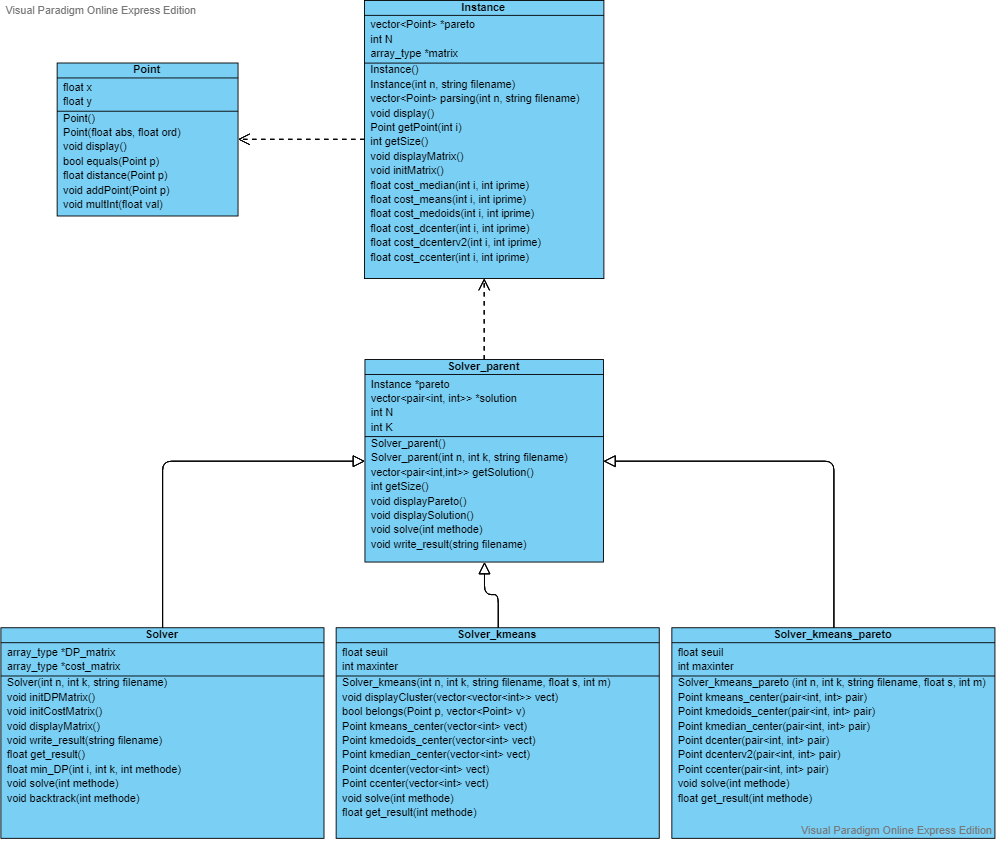
\includegraphics[scale=0.5]{TER.png}

\subsection{Réutilisation du code}

Notre code a été pensé programmation objet et comporte donc plusieurs classes : Point.cpp permet de représenter un point avec ses coordonnées en attribut. Instance.cpp permet de représenter notre front de pareto sous la forme d'un vecteur de points. Solver\_parent.cpp est la classe mère de nos solvers et n'implémente pas la fonction principale solve, elle ne doit pas etre utilisée. Solver.cpp est le sovler principal utilisant la programmation dynamique. Solver\_kmeans.cpp est un solver utilisant l'algorithme de Lloyd générique. Solver\_kmeans\_pareto.cpp est un solver utilisant l'algorithme de Lloyd optimisé pour un front de pareto.\\

Le principal fichier exécutable généré par notre code est test\_final. Cet exécutable ne sera jamais exécuté seul mais sera utilisé par le programme python test.py qui lancera ce programme et récuperera ses résultats, grace au module python subprocess. Un makefile est présent dans le dossier src, pour compiler la partie C++ il suffit donc de se placer dans ce dossier et appeler make. Pour exécuter le code il faut exécuter le programme python test.py, qui prend 7 arguments : \\
directory : le répertoire dans lequel aller chercher les données, qui correspond aussi à la méthode de génération des données.\\
N : le nombre de points des instances que l'on va générer.\\
K : le nombre de clusters que l'on veut considérer.\\
method : la méthode de calcul de coût de clustering utilisée par nos solvers (median, means...).\\
seuil : le paramètre de seuil utilisé dans l'algorithme de Lloyd.\\
maxiter : le paramètre d'itérations maximum utilisé dans l'algorithme de Lloyd.\\
nb\_inst : le nombre d'instances de données que l'on veut créer pour ces paramètres.\\
Le programme python va exécuter le programme C++ test\_final et récupérer ses sorties consoles, puis écrire les résultats dans un fichier csv, dont le nom est de la forme "Result\_directory\_method\_date.csv".

\section{References}
\scriptsize

$\bullet$ {N. Dupin, E. Talbi and F. Nielsen},
{\emph{Clustering in a 2-dimensional Pareto Front: p-median and p-center are solvable in polynomial time}},
{arXiv preprint}, \url{https://arxiv.org/pdf/1806.02098.pdf },
{2018}.\\
$\bullet$ {N. Dupin, F. Nielsen and E. Talbi}, 
\emph{Dynamic programming heuristic for k-means clustering in a 2-dimensional Pareto Front},
META 2018, 7th International Conference on Metaheuristics and Nature Inspired Computing,
available online, 2018.

\end{document}